\tikzstyle{white} = [circle, draw, fill=white!25, minimum size=10pt]
\tikzstyle{black} = [circle, draw, fill=black!25, minimum size=10pt]
\tikzstyle{edge} = [draw, thick, >=latex]

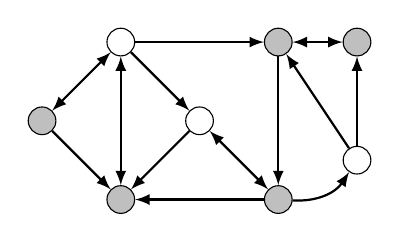
\begin{tikzpicture}
	\node[white] (0) at (-2, 0) {};
	\node[black] (1) at (0, 0) {};
	\node[black] (2) at (0, -2) {};
	\node[black] (3) at (-2, -2) {};
	\node[white] (4) at (-1, -1) {};
	\node[black] (5) at (-3, -1) {};
	\path[edge, ->] (0) -- (1);
	\path[edge, ->] (1) -- (2);
	\path[edge, ->] (2) -- (3);
	\path[edge, <->] (3) -- (0);
	\path[edge, ->] (0) -- (4);
	\path[edge, <->] (4) -- (2);
	\path[edge, ->] (4) -- (3);
	\path[edge, <->] (5) -- (0);
	\path[edge, ->] (5) -- (3);

	\node[black] (a) at (1, 0) {};
	\node[white] (e) at (1, -1.5) {};
	\path[edge, <->] (1) -- (a);
	\path[edge, <-] (1) -- (e);
	\path[edge, ->] (2) edge [bend right = 30] (e);

	\path[edge, ->] (e) -- (a);
\end{tikzpicture}
